\subsection{Feature Extraction} \label{subsec:feature-extraction}

The feature extraction module receives a multi-channel audio signal of a fixed
length and outputs a \emph{feature frame}. Which is defined as the group of
vectors of features extracted from a finite number of samples. One vector per
\emph{extractor} used. \Cref{fig:datasets-frames} illustrates how an audio
signal is divided into frames.

\begin{figure}
    \centering
    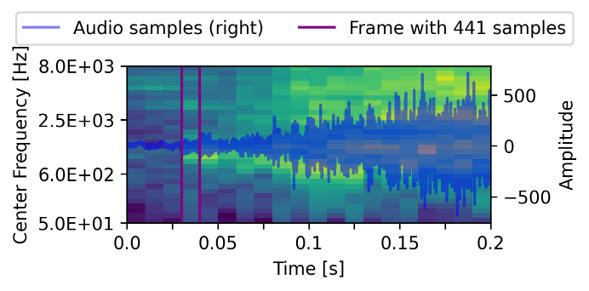
\includegraphics[width=\linewidth]{\subdir/frames.png}
    \caption[Audio frames]{Audio signal (in {\color{blue} blue}) over its
        features extracted from frames with a duration of 10 ms with a single
        \nameref{subsubsec:gammatone-filterbank} extractor.}
    \label{fig:datasets-frames}
\end{figure}

The term \emph{extractor} will be used to abstract the system used to extract
features from audio data. This work opts to use a feature extractor based on
\nameref{subsubsec:gammatone-filterbank} since the performance of
classification systems relying on Mel Frequency Cepstrum Coefficients is
greatly reduced in the presence of noise \cite{marchegiani2018a}.

\subsubsection*{Gammatone filterbanks} \label{subsubsec:gammatone-filterbank}

An approximation to the human cochlear frequency selectivity originally
introduced in \cite{GTF1998}. Time-independent features are obtained by
filtering the audio waveform with a bank of gammatone band-pass filters. The
impulse response of a gammatone filter centered at frequency $f_c$ is given by
\cref{eq:gammatone-filter-impulse}, where $n$ indicates the order of the filter
which largely determines the slope of the filter's skirts; and $b$ is the
bandwidth of the filter and largely determines the duration of the impulse
response; $a$ is the amplitude and $\phi$ is the phase.

\begin{equation}
    g(t, f_c) = a t^{n-1}e^{-2 \pi b t} \cos{2 \pi f_c t + \phi}
    \label{eq:gammatone-filter-impulse}
\end{equation}

This work implements a bank of fourth order gammatone filters with its
corresponding bandwidth $b$ of 1.019 ERB where ERB is the equivalent
rectangular bandwidth scale \cite{GLASBERG1990103}. It is based on a Matlab MEX
function implemented in C by \citeauthor{CorrelogramMa2007}
\cite{CorrelogramMa2007}, which at the same time is based on
\citeauthor{Cooke1993ModellingAP}'s Ph.D work \cite{Cooke1993ModellingAP}. The
filters are linearly distributed over a predefined frequency range on the ERB
scale. The number of filters used is equivalent to the number of features to be
extracted. 